\documentclass[14pt]{extbook}
\usepackage{multicol, enumerate, enumitem, hyperref, color, soul, setspace, parskip, fancyhdr} %General Packages
\usepackage{amssymb, amsthm, amsmath, latexsym, units, mathtools} %Math Packages
\everymath{\displaystyle} %All math in Display Style
% Packages with additional options
\usepackage[headsep=0.5cm,headheight=12pt, left=1 in,right= 1 in,top= 1 in,bottom= 1 in]{geometry}
\usepackage[usenames,dvipsnames]{xcolor}
\usepackage{dashrule}  % Package to use the command below to create lines between items
\newcommand{\litem}[1]{\item#1\hspace*{-1cm}\rule{\textwidth}{0.4pt}}
\pagestyle{fancy}
\lhead{Makeup Progress Quiz 3}
\chead{}
\rhead{Version B}
\lfoot{1648-1753}
\cfoot{}
\rfoot{Summer C 2021}
\begin{document}

\begin{enumerate}
\litem{
Determine the appropriate model for the graph of points below.
\begin{center}
    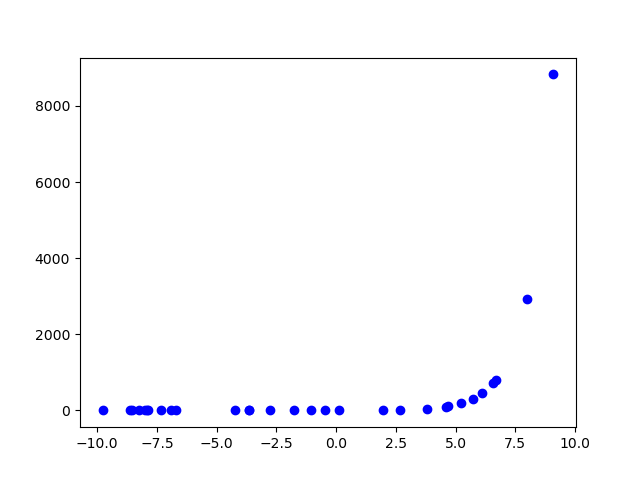
\includegraphics[width=0.5\textwidth]{../Figures/identifyModelGraph12B.png}
\end{center}
\begin{enumerate}[label=\Alph*.]
\item \( \text{Exponential model} \)
\item \( \text{Logarithmic model} \)
\item \( \text{Linear model} \)
\item \( \text{Non-linear Power model} \)
\item \( \text{None of the above} \)

\end{enumerate} }
\litem{
For the scenario below, use the model for the volume of a cylinder as $V = \pi r^2 h$.
\begin{center}
    \textit{ Pringles wants to add 27 \text{percent} more chips to their cylinder cans and minimize the design change of their cans. They've decided that the best way to minimize the design change is to increase the radius and height by the same percentage. What should this increase be? }
\end{center}
\begin{enumerate}[label=\Alph*.]
\item \( \text{About } 3 \text{ percent} \)
\item \( \text{About } 14 \text{ percent} \)
\item \( \text{About } 13 \text{ percent} \)
\item \( \text{About } 8 \text{ percent} \)
\item \( \text{None of the above} \)

\end{enumerate} }
\litem{
For the scenario below, use the model for the volume of a cylinder as $V = \pi r^2 h$.
\begin{center}
    \textit{ Pringles wants to add 27 \text{percent} more chips to their cylinder cans and minimize the design change of their cans. They've decided that the best way to minimize the design change is to increase the radius and height by the same percentage. What should this increase be? }
\end{center}
\begin{enumerate}[label=\Alph*.]
\item \( \text{About } 8 \text{ percent} \)
\item \( \text{About } 13 \text{ percent} \)
\item \( \text{About } 3 \text{ percent} \)
\item \( \text{About } 14 \text{ percent} \)
\item \( \text{None of the above} \)

\end{enumerate} }
\litem{
Determine the appropriate model for the graph of points below.
\begin{center}
    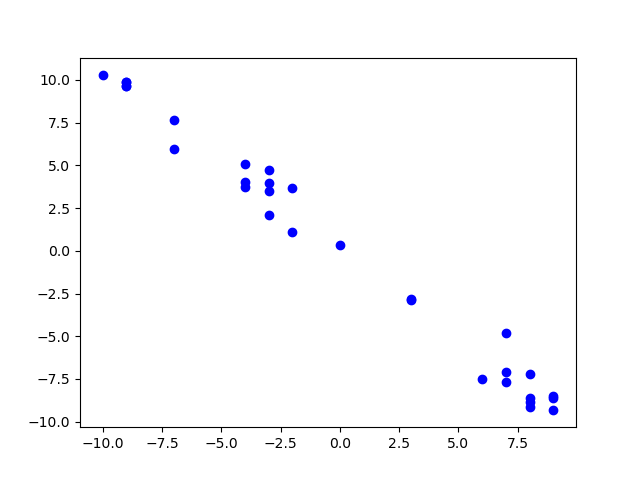
\includegraphics[width=0.5\textwidth]{../Figures/identifyModelGraph12CopyB.png}
\end{center}
\begin{enumerate}[label=\Alph*.]
\item \( \text{Non-linear Power model} \)
\item \( \text{Linear model} \)
\item \( \text{Exponential model} \)
\item \( \text{Logarithmic model} \)
\item \( \text{None of the above} \)

\end{enumerate} }
\litem{
Solve the modeling problem below, if possible.
\begin{center}
    \textit{ A new virus is spreading throughout the world. There were initially 3 many cases reported, but the number of confirmed cases has quadrupled every 1 days. How long will it be until there are at least 100000 confirmed cases? }
\end{center}
\begin{enumerate}[label=\Alph*.]
\item \( \text{About } 5 \text{ days} \)
\item \( \text{About } 8 \text{ days} \)
\item \( \text{About } 11 \text{ days} \)
\item \( \text{About } 6 \text{ days} \)
\item \( \text{There is not enough information to solve the problem.} \)

\end{enumerate} }
\litem{
Solve the modeling problem below, if possible.
\begin{center}
    \textit{ In CHM2045L, Brittany created a 24 liter 14 percent solution of chemical $\chi$ using two different solution percentages of chemical $\chi$. When she went to write her lab report, she realized she forgot to write the amount of each solution she used! If she remembers she used 8 percent and 19 percent solutions, what was the amount she used of the 8 percent solution? }
\end{center}
\begin{enumerate}[label=\Alph*.]
\item \( 11.65 liters \)
\item \( 12.00 liters \)
\item \( 13.09 liters \)
\item \( 10.91 liters \)
\item \( \text{There is not enough information to solve the problem.} \)

\end{enumerate} }
\litem{
Solve the modeling problem below, if possible.
\begin{center}
    \textit{ In CHM2045L, Brittany created a 27 liter 27 percent solution of chemical $\chi$ using two different solution percentages of chemical $\chi$. When she went to write her lab report, she realized she forgot to write the amount of each solution she used! If she remembers she used 10 percent and 36 percent solutions, what was the amount she used of the 36 percent solution? }
\end{center}
\begin{enumerate}[label=\Alph*.]
\item \( 12.68 liters \)
\item \( 9.35 liters \)
\item \( 13.50 liters \)
\item \( 17.65 liters \)
\item \( \text{There is not enough information to solve the problem.} \)

\end{enumerate} }
\litem{
For the scenario below, find the variation constant $k$ of the model (if possible).
\begin{center}
    \textit{ In an alternative galaxy, the square of the time, $T$ (Earth years), required for a planet to orbit Sun $\chi$ increases as the square of the distance, $d$ (AUs), that the planet is from Sun $\chi$ increases. For example, when Ea's average distance from Sun $\chi$ is 7, it takes 100 Earth days to complete an orbit. }
\end{center}
\begin{enumerate}[label=\Alph*.]
\item \( k = 490000.000 \)
\item \( k = 4.028 \)
\item \( k = 204.082 \)
\item \( k = 3.780 \)
\item \( \text{Unable to compute the constant based on the information given.} \)

\end{enumerate} }
\litem{
For the information provided below, construct a linear model that describes her total costs, $C$, as a function of the number of months, $x$ she is at UF. 
\begin{center}
    \textit{ Aubrey is a college student going into her first year at UF. She will receive Bright Futures, which covers her tuition plus a \$600 educational expense each year. Before college, Aubrey saved up \$10000. She knows she will need to pay \$1200 in rent a month, \$80 for food a week, and \$40 in other weekly expenses. }
\end{center}
\begin{enumerate}[label=\Alph*.]
\item \( C(x) = 1320 x \)
\item \( C(x) = 10600 \)
\item \( C(x) = 1320 \)
\item \( C(x) = 10600 x \)
\item \( \text{None of the above.} \)

\end{enumerate} }
\litem{
Solve the modeling problem below, if possible.
\begin{center}
    \textit{ A new virus is spreading throughout the world. There were initially 4 many cases reported, but the number of confirmed cases has tripled every 5 days. How long will it be until there are at least 10000 confirmed cases? }
\end{center}
\begin{enumerate}[label=\Alph*.]
\item \( \text{About } 19 \text{ days} \)
\item \( \text{About } 36 \text{ days} \)
\item \( \text{About } 40 \text{ days} \)
\item \( \text{About } 20 \text{ days} \)
\item \( \text{There is not enough information to solve the problem.} \)

\end{enumerate} }
\end{enumerate}

\end{document}